\input qpd-bootstrap

\begin{problem}{20260803}
  \meta{name}{The Trolley Problem}
  \meta{setter}{Andy He}
  \meta{score}{6}
  \meta{topic}{mechanics}
  \meta{difficulty}{2}
  \meta{tags}{mechanics, rotation, rolling, energy}

Today, SM-senior 黄瑞宣 was kidnapped by the evil Professor 孙笑川. The wicked Emperor has decided to make our great SM-senior 黄瑞宣 solve a problem that has long troubled humanity --- and, in doing so, to steal 李文亚's Nobel Prize. After weighing many awards, Professor 孙笑川 concluded that only the Nobel Prize in Physics could suppress 李文亚's white-body biology theory, so he resolved to have 黄瑞宣 solve a physics problem that has baffled all of humankind: the Trolley Problem. 黄瑞宣 had to choose between securing a pentakill for the ace elite and completing an online solo kill. Under Professor 孙笑川's coercion, and with the weight of past memories flooding back, 黄瑞宣 transformed on the spot into the Identity V character 破轮 (whose appearance is shown below).

\begin{center}
  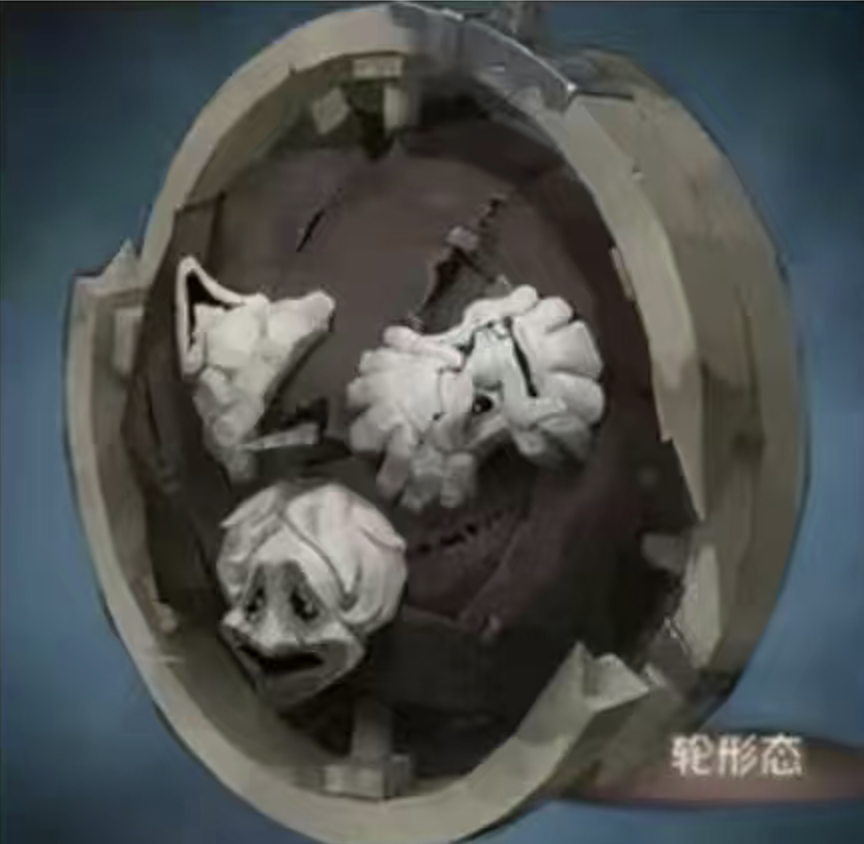
\includegraphics[width=0.45\linewidth]{assets/20260803-1.png}
\end{center}

…and crushed Professor 孙笑川 to death, bringing his sinful life to an end.

Treat Professor 孙笑川 as a hemisphere of radius $r$ lying on a plane. 黄瑞宣, having become 破轮, has radius $R$, mass $M$, and moment of inertia $I = \tfrac12 M R^{2}$, and has speed $v$ at the instant he crushes into Professor 孙笑川.

\begin{questions}
  \item Find the kinetic energy lost in rolling over Professor 孙笑川.
  \item Find the minimum initial speed $v$ for 黄瑞宣 to just barely roll over Professor 孙笑川.
\end{questions}

\end{problem}

\begin{solution}{20260803}

破轮 is a uniform disk, so its moment of inertia is $I = \tfrac12 M R^{2}$. When rolling without slipping on the ground, the total kinetic energy is the sum of translational and rotational parts:
\[
E_k = \tfrac12 M v^{2} + \tfrac12 I \omega^{2}
    = \tfrac12 M v^{2} + \tfrac12 \cdot \tfrac12 M R^{2}\!\left(\frac{v}{R}\right)^{2}
    = \tfrac34 M v^{2}.
\]

\textbf{Q1. Kinetic energy lost.} As 破轮 rolls from the ground (centre of mass at height $R$) up to the top of the hemisphere, its centre of mass rises to $R+r$, an increase of $\Delta h = r$. For ideal rolling without slipping there is no dissipation, so the kinetic energy lost is entirely converted into gravitational potential energy:
\[
\boxed{\Delta E_k = M g r}.
\]

\textbf{Q2. Minimum initial speed.} To \emph{just barely} roll over Professor 孙笑川, 破轮 arrives at the top of the hemisphere with zero kinetic energy. By conservation of mechanical energy,
\[
\tfrac34 M v_{\min}^{2} = M g r
\;\Longrightarrow\;
\boxed{v_{\min} = \sqrt{\tfrac{4}{3} g r}}.
\]

\end{solution}

\input qpd-end
